\documentclass[a4paper,12pt,oneside]{article}
\usepackage{amsmath}
%\usepackage{mathtools}
\usepackage{caption}
\usepackage{mathptmx}
\usepackage{graphicx}
\usepackage[margin=1.0in]{geometry}
\usepackage{float}
\usepackage{setspace}
\usepackage{chngcntr}
\usepackage{fancyhdr}
\usepackage{etoolbox}
\patchcmd{\thebibliography}{\section*{\refname}}{}{}{}
\pagestyle{fancy}
\fancyhf{}
\rfoot{\thepage}
%\renewcommand{\headrulewidth}{0.0pt}
%\renewcommand{\footrulewidth}{0.0pt}

\begin{document}
\thispagestyle{empty}
%\pagenumbering{gobble}
\begin{center}

\large{\textbf{Facial emotion recognition in real-time and static
images}
\setlength{\baselineskip}{1.5\baselineskip}}
\\

\vspace{5mm}
\textbf{SEMINAR REPORT}
\\
\vspace{3mm}
Submitted in the partial fulfilment of the award of the degree
of
\vspace{3mm}
\\
\textbf{Bachelor of Technology}
\\
\vspace{3mm}
in
\\
\vspace{3mm}
\textbf{Computer Science and Engineering}
\\
\vspace{3mm}
of
\\
\vspace{3mm}
\textbf{APJ Abdul Kalam Technological University}
\\
\vspace{3mm}
by
\\
\vspace{3mm}
\textbf{Manimaran N}
\\
\vspace{5mm}
\begin{figure}[H]
	\centering
	
\includegraphics{ceclogo.png}
\end{figure}
\vspace{25mm}
\textbf{November, 2018}
\vspace{8mm}
\\
\vspace{2mm}
Department of Computer Engineering
\\
\vspace{2mm}
College of Engineering, Chengannur, Kerala -689121
\\
\vspace{2mm}
Phone: (0479) 2454125, 2451424; Fax: (0479) 2451424
\\


\end{center}

\newpage
\thispagestyle{empty}
\begin{center}
\setlength{\baselineskip}{1.5\baselineskip}
{\large\textbf{COLLEGE OF ENGINEERING, CHENGANNUR}}
\\
{\large\textbf{KERALA}}
\\
\begin{figure}[H]
\centering

\includegraphics{ceclogo.png}
\end{figure}
\setlength{\baselineskip}{1.5\baselineskip}
\textbf{Department of Computer Engineering}
\\
\textbf{CERTIFICATE}
\\
This is to certify that the seminar entitled
\\
\textbf{Facial emotion recognition in real-time and static
images}
\\
Submitted by
\\
\textbf{Manimaran N}
\\
is a bonafide record of the work done by him.
\end{center}
\vspace{20mm}
\vspace{25ex}
%\textbf{Mrs.Shiny}
\hspace{55ex}
%\textbf{Dr. Smitha Dharan}
\\
\vspace{2ex}
\hspace{0ex}
\textbf{
Co-ordinator}
\hspace{20ex}
\textbf{
Guide}
\hspace{16ex}
\textbf{
Head of The Department}
\newpage
\pagenumbering{roman}


\renewcommand{\headrulewidth}{0.0pt}
\renewcommand{\footrulewidth}{0.0pt}



\begin{center}
\large{\textbf{ACKNOWLEDGEMENT}}
\end{center}
\vspace{6ex}
\setlength{\baselineskip}{1.5\baselineskip}

\paragraph{}
I am greatly indebted to God Almighty for being the guiding light throughout with his
abundant grace and blessings that strengthened me to do this endeavour with confidence.
\paragraph{}
I express my heartfelt gratitude towards \textbf{Dr. Jacob Thomas V.}, Principal, College
of Engineering Chengannur for extending all the facilities required for doing my seminar.
I would also like to thank \textbf{Dr. Smitha Dharan}, Head, Department of Computer
Engineering, for providing constant support and encouragement.
\paragraph{}
Now I extend my sincere thanks to my seminar co-ordinators \textbf{Mrs.Shiny B}, Assistant
Professor in Computer Engineering , \textbf{Mrs.C Jyothirmayi Devi}, Assistant
Professor in Computer Engineering , \textbf{Ms. Archana Vijayan} , Assistant
Professor in Computer Engineering and \textbf{Ms. Arathy U P} , Assistant
Professor in Computer Engineering for guiding me in my work and providing timely
advices and valuable suggestions.
\paragraph{}
Last but not the least, I extend my heartfelt gratitude to my parents and friends for
their support and assistance.	

\pagenumbering{gobble}
\newpage

\begin{center}
\large{\textbf{ABSTRACT}}
\end{center}
\vspace{6ex}
\paragraph{}

Facial expressions are a form of nonverbal
communication. Various studies have been done for the
classification of these facial expressions. There is strong
evidence for the universal facial expressions of eight
emotions which include: neutral happy, sadness, anger,
contempt, disgust, fear, and surprise. So it is very
important to detect these emotions on the face as it has
wide applications in the field of Computer Vision and
Artificial Intelligence. These fields are researching on
the facial emotions to get the sentiments of the humans
automatically. In Robotics, emotions classification can
be used to enhance human-robot interactions since the
robot is capable of interpreting a human reaction. In
this paper, the emotion detection has been done in both
real-time and static images. In this project, we have used
the Cohn-Kanade Database (CK) and the Extended
Cohn-Kanade (CK+) database, which comprises many
static images 640 x 400 pixels and for the real-time using
the webcam. The target expression for each sequence in
the datasets are fully FACS (Facial action coding
system) coded and emotion labels have been revised and
validated [3]. So for emotion recognition initially we
need to detect the faces by using HAAR filter from
OpenCV in the static images or in the real-time videos.
Once the face is detected it can be cropped and processed
for further detection of facial landmarks. Then using
facial landmarks the datasets are trained using the
machine learning algorithm (Support Vector Machine)
and then classified according to the eight emotions.
Using SVM we were getting the accuracy of around
93.7\% . These facial landmarks can be modified for
getting better accuracy.
\setlength{\baselineskip}{1.0\baselineskip}
\newpage
\begin{center}
\tableofcontents
\end{center}


\newpage
\thispagestyle{plain}
\begin{center}
\vspace{5mm}
\listoffigures
\vspace{5mm}

\end{center}





\newpage
\rfoot{\thepage}

\lhead{\textit{Facial emotion recognition in real-time and static
images}}

\lfoot{\textit{College of Engineering, Chengannur}}

\rfoot{\thepage}

\renewcommand{\headrulewidth}{0.0pt}
\renewcommand{\footrulewidth}{0.0pt}




\renewcommand{\headrulewidth}{0.0pt}
\renewcommand{\footrulewidth}{0.0pt}



\section{INTRODUCTION}
\pagenumbering{arabic}
\paragraph{}
An emotion can be defined as the physiological and
mental state which is subjective and private. It involves
a lot of behaviors, actions, thoughts, and feelings. In the
field of computer vision these emotions, play an
important role for different research purposes. In this
project, the images datasets were organized properly and
then sorted accordingly. Then the face was detected in
all the images using the Haar filters [20] in OpenCV as
it has few face recognized classes and then detect, crop
and save faces. The classification is done using the
supervised learning (SVM) [15] in this project as it gave
better accuracy. The training and classification sets were
created and we randomly sample and train on 80\% of the
data and classify the remaining 20\%. This whole work
was done on the Cohn-Kanade datasets of static images.
\paragraph{}
This study has also been extended in the real time as well
in which like we detect the emotions in the static images.
Now the webcam will be running a video and the faces
are going to be detected in the frames according to the
facial landmarks which will contain the eyes, eyebrows,
nose, mouth, corners of the face. Then the features were
extracted from these facial landmarks (dots) faces which
will be utilized for the detection of the facial emotions. This was optimized by calculating the centre of
gravity of all these dots and calculating the distance
between the centre of gravity and the corresponding dots.
After the extraction of these features, the machine
learning algorithms were applied for training and
classifying the different emotions. Then the
performance was evaluated in the real-time and the static
images.


\newpage
\section{LITERATURE REVIEW}
\paragraph{•}
\textbf{Facial Emotion Recognition:}
\textit{Ma Xiaoxi, Lin Weisi }
in This paper has implemented several learning methods:
SVM and DBM, which are all excellent methods in general
and the aim is to construct the prediction system which is
most suitable to the challenge. Comparing the experiment
results of different prediction systems, the best performance
of Occurrence Detection of AUs is obtained by emotional facial classification system with SVM. This paper mainly
focuses on the implementation and caparison of different
learning methods. For future work, the prediction results of
facial data and audio data should be merged, and also the
prediction results of different learning methods should also
be merged to enhance the performance of the prediction
system. Besides, there are numerous decision fusion methods,
and only the simple fusion is implemented in this paper. For
future work, more fusion methods need to be learned for
their principles, and more fusion methods need to be
implemented and compared.
\paragraph{•}
\textbf{An Efficient Method to Face and Emotion Detection:}
\textit{Dolly Reney,Dr.Neeta Tripaathi }
In this paper they have implemented an efficient method to detect
face and emotion of the person. For detecting the face from
the image we use the well known Viola Jones face detection
method and for detecting voice features we used Mel
frequency components of the human voice. By using KNN
classifier algorithm is used to face and emotion
reorganization of the person. Experimental results show the
efficiency of the proposed face and emotion reorganization
system is 94.5\% to 97 \%.
\paragraph{•}
\textbf{Emotion Recognition From Facial Expressions and
Its Control Using Fuzzy Logic:}
\textit{Aruna Chakraborty, Amit Konar:-}
in This paper presents a fuzzy relational approach to
human emotion recognition from facial expressions and its control.
The proposed scheme uses external stimulus to excite specific
emotions in human subjects whose facial expressions are analyzed
by segmenting and localizing the individual frames into regions
of interest. Selected facial features such as eye opening, mouth
opening, and the length of eyebrow constriction are extracted
from the localized regions, fuzzified, and mapped onto an emotion
space by employing Mamdani-type relational models. A scheme
for the validation of the system parameters is also presented. This
paper also provides a fuzzy scheme for controlling the transition
of emotion dynamics toward a desired state. Experimental results
and computer simulations indicate that the proposed scheme for
emotion recognition and control is simple and robust, with good
accuracy.
\paragraph{•}
\textbf{An analysis of facial expression recognition under partial
facial image occlusion}
\textit{Irene Kotsia *, Ioan Buciu, Ioannis Pitas }
In this paper, an analysis of the effect of partial occlusion on facial expression recognition is investigated. The classification from partially
occluded images in one of the six basic facial expressions is performed using a method based on Gabor wavelets texture information
extraction, a supervised image decomposition method based on Discriminant Non-negative Matrix Factorization and a shape-based
method that exploits the geometrical displacement of certain facial features. We demonstrate how partial occlusion affects the above
mentioned methods in the classification of the six basic facial expressions, and indicate the way partial occlusion affects human observers
when recognizing facial expressions. An attempt to specify which part of the face (left, right, lower or upper region) contains more discriminant
information for each facial expression, is also made and conclusions regarding the pairs of facial expressions misclassifications
that each type of occlusion introduces, are drawn.
\newpage
\section{MATERIALS AND DATASETS}
\paragraph{}
We have used the Cohn-Kanade Database (CK) and the
Extended Cohn-Kanade Database (CK+) of the Carnegie
Mellon University (CMU) which contains the sequence
of static images from neutral to a particular emotion. In
this project, we have implemented it in Python. OpenCV
(open source computer vision) was required as this
project is based on the computer vision. For the Real-
time webcam is required which is going to record the
video and the facial emotions will be detected. We have
used python 2.7 (Anaconda + Jupyter notebook is a nice
combo-package). Dlib library was installed (a C++
library for extracting the facial landmarks). CMake and
Boost-Python were also used in this research-based
project.
\paragraph{}









\subsection{Cohn-Kanade Database (CK)}

\paragraph{}
The Cohn-Kanade AU-Coded Facial Expression Database is for research in automatic facial image analysis and synthesis and for perceptual studies.which contains the sequence of static images from neutral to a particular emotion.  the initial release, includes 486 sequences from 97 posers. Each sequence begins with a neutral expression and proceeds to a peak expression. The peak expression for each sequence in fully FACS (Ekman, Friesen, & Hager, 2002; Ekman & Friesen, 1979) coded and given an emotion label. The emotion label refers to what expression was requested rather than what may actually have been performed. 



\subsection{Extended Cohn-Kanade Database (CK+)}
\paragraph{}
In 2000, the Cohn-Kanade (CK) database was released for the purpose of promoting research into automatically detecting individual facial expressions. Since then, the CK database has become one of the most widely used test-beds for algorithm development and evaluation. During this period, three limitations have become apparent: 1) While AU codes are well validated, emotion labels are not, as they refer to what was requested rather than what was actually performed, 2) The lack of a common performance metric against which to evaluate new algorithms, and 3) Standard protocols for common databases have not emerged. As a consequence, the CK database has been used for both AU and emotion detection (even though labels for the latter have not been validated), comparison with benchmark algorithms is missing, and use of random subsets of the original database makes meta-analyses difficult. To address these and other concerns, we present the Extended Cohn-Kanade (CK+) database. The number of sequences is increased by 22\% and the number of subjects by 27\%. The target expression for each sequence is fully FACS coded and emotion labels have been revised and validated. In addition to this, non-posed sequences for several types of smiles and their associated metadata have been added. We present baseline results using Active Appearance Models (AAMs) and a linear support vector machine (SVM) classifier using a leave-one-out subject cross-validation for both AU and emotion detection for the posed data. The emotion and AU labels, along with the extended image data and tracked landmarks are available now.





\subsection{OpenCV (Open Source Computer Vision Library)}
\paragraph{}
OpenCV (Open Source Computer Vision Library) is an open source computer vision and machine learning software library. OpenCV was built to provide a common infrastructure for computer vision applications and to accelerate the use of machine perception in the commercial products. Being a BSD-licensed product, OpenCV makes it easy for businesses to utilize and modify the code.

\paragraph{}
The library has more than 2500 optimized algorithms, which includes a comprehensive set of both classic and state-of-the-art computer vision and machine learning algorithms. These algorithms can be used to detect and recognize faces, identify objects, classify human actions in videos, track camera movements, track moving objects, extract 3D models of objects, produce 3D point clouds from stereo cameras, stitch images together to produce a high resolution image of an entire scene, find similar images from an image database, remove red eyes from images taken using flash, follow eye movements, recognize scenery and establish markers to overlay it with augmented reality, etc. OpenCV has more than 47 thousand people of user community and estimated number of downloads exceeding 14 million. The library is used extensively in companies, research groups and by governmental bodies.

\subsection{FACS (Facial Action Coding System)}
\paragraph{}
Facial Action Coding System is a system to taxonomize human facial movements by their appearance on the face, based on a system originally developed by a Swedish anatomist named Carl-Herman Hjortsjö. It was later adopted by Paul Ekman and Wallace V. Friesen, and published in 1978.Movements of individual facial muscles are encoded by FACS from slight different instant changes in facial appearance.[4] It is a common standard to systematically categorize the physical expression of emotions, and it has proven useful to psychologists and to animators. Due to subjectivity and time consumption issues, FACS has been established as a computed automated system that detects faces in videos, extracts the geometrical features of the faces, and then produces temporal profiles of each facial movement.

\subsection{k-means clustering }
\paragraph{}
K-means clustering is a type of unsupervised learning, which is used when you have unlabeled data (i.e., data without defined categories or groups). The goal of this algorithm is to find groups in the data, with the number of groups represented by the variable K. The algorithm works iteratively to assign each data point to one of K groups based on the features that are provided. Data points are clustered based on feature similarity. The results of the K-means clustering algorithm are:
 
\begin{itemize}
   \item The centroids of the K clusters, which can be used to label new data
   \item Labels for the training data (each data point is assigned to a single cluster)
\end{itemize}
Rather than defining groups before looking at the data, clustering allows you to find and analyze the groups that have formed organically. The "Choosing K" section below describes how the number of groups can be determined.  

Each centroid of a cluster is a collection of feature values which define the resulting groups. Examining the centroid feature weights can be used to qualitatively interpret what kind of group each cluster represents.  



\paragraph{}
\textbf{Keywords:}  FACS, HAAR, Support vector machine,
OpenCV, k-means clustering.

\newpage
\section{METHODOLOGY}
\subsection{In Static Images}

\subsubsection{Data organization}
\paragraph{}
A face consists of some features on it which play an
important role in the detection of the emotions on it. The
emotion recognition system is divided into 3 stages: face
detection, feature extraction, and emotion classification.
We have encoded our eight emotions in the datasets as
{0= happy, 1=sadness, 2=fear, 3=anger, 4=surprise,
5=disgust, 6=contempt, 7=neutral}. Initially, the faces
are detected in all the sequences of the Cohn-Kanade
Database. First, we have organized the dataset by
preparing two folders called “emotions source” and
“images source” in the directory we are working and put
all folders containing the text files with FACS in a folder
called “emotions source” and put the folders containing
the images in a folder called “images source”. We have
also created a folder named “sorted images set”, to
collect our sorted emotion images. Within this folder, we
have folders for the emotion labels (“happy”, “disgust”,
etc.). Each image sequence consists of the development
of an emotional expression, starting from a neutral face
and ending with some particular emotion. So, from each
image sequence, our focus is to extract two images that
are one neutral (the first image) and one with an
emotional expression (the last image) in the sequence.

\subsubsection{Extracting Faces}
\paragraph{}
The classifier will work properly if the images contain
only the faces so the images were processed accordingly
for the detection of the faces and then were converted to
grayscale and were cropped and were stored in some
specific folder [7]. We have used a HAAR filter from
OpenCV for automatic detection of faces. As OpenCV
contains 4 pre-trained classifiers, so it is better we detect
as many faces as possible. We have Created another
folder called “Extracted faces datasets”, and subfolders
within this folder for each emotion (“sadness”, “happy”,
etc.).

\subsubsection{Training and classification}
\paragraph{}
The dataset has been organized and is ready to be
recognized, but initially, we need to actually train the
classifier what particular emotions look like. The
approach we have used is to split the complete dataset
into a training set and a classification set. We use the
training set to teach the classifier to recognize the labels
to be predicted, and used the classification set to estimate
the performance of the classifier. After creating the
training and classification set, we randomly sample and
train on 80\% of the data and classify the remaining 20\%,
and repeat the process 20 times. After training the
fisher face classifier the emotions were predicted.


\subsection{In Real-Time}
\paragraph{}

In real time the emotions can also be detected but it
becomes quite complex when compared to the static
images as in the real-time the webcam is recording a
video which is a collection of many frames, not just a
single frame. In this case, we have used the Facial
Landmarks approach to detect emotions,
continuously which is more robust and powerful than the
fisherface classifier which was used in the
sequences of static images but it also required some more
features and modules. After installing the Dlib libraries,
CMake and boost python build the libraries.

\subsubsection{Testing the landmark detector}
\paragraph{}
Initially, we need to operate the webcam on the computer
which is going to record the real-time video. The faces
will be detected in each frame of the webcam video and
then the further processing will be done on those
detected faces. In real-time also we have used OpenCV
to operate webcam. Then after that, the image is
processed by converting to grayscale, optimising the
contrast with an adaptive histogram equalization.

\subsubsection{Extracting features from the faces}
\paragraph{}
In the feature extraction stage, the faces detected in the
previous stage are further processed for identification of
eye, eyebrows, nose, corner of face and mouth regions.
Initially, the likely Y coordinates of the eyes were
identified with the use of the horizontal projection. Then
the areas around the y coordinates were processed to
identify the exact regions of the features. Finally, a
corner point detection algorithm was used to obtain the
required corner points from the feature regions.

\paragraph{}
This will result in a lot of dots on the faces in the webcam
video outlining the shape and all the “moveable parts”. The latter is, of course, important because it is what
makes emotional expressions possible. These dots are
very important for the extraction of the features for the
training and classification using the Machine learning
algorithms. Then we implemented the ways to transform
these nice dots overlaid on faces in the webcam video
into features to feed the classifier. Features are small
information that is used to describe the object or object
state that we are trying to classify into
different categories. The facial landmarks from the
image material tell about the position of all the “moving
parts” of the depicted face, the things we need to express
an emotion.

\paragraph{}
We calculated the coordinates of all facial landmarks
[16]. These coordinates are the first collection of
features, and this might be the end of the road. We
derived other measures from this that will inform the
classifier more about what is being calculated on the
faces detected. We tried to extract more information
from what we have. Feature generation is always a better
way for classification because it brings you closer to the
actual data [16]. The coordinates may change as my face
moves to different parts of the frame. I could be
expressing the same emotion in the top left of an image
as in the bottom right of another image, but the resulting
coordinate matrix would express different numerical
ranges. To get rid of these numerical differences
originating from faces in different places of the image we
normalized the coordinates between 0 and 1. This was
done by the following equation (1) :

\[X_{norm}=\frac{X-X_{min}}{X_{max}-X_{min}}\]

\paragraph{}
The more precise way which we have implemented to
calculate the position of all points relative to each other.
To do this we calculated the mean of both axes, which
results in the point coordinates of the sort-of “centre of
gravity” of all face landmarks. We can then get
the position of all points relative to this central
point. Note that each line has both a magnitude (distance
between both points) and a direction (angle relative to
image where horizontal=0°), in other words, a
vector. The problem we need to fix is that Faces may be
tilted in the webcam which might confuse the classifier.
We can correct for this rotation by assuming that the
bridge of the nose for most people is more or less
straight, and offset all calculated angles by the angle of
the nose bridge. This rotates the entire vector array so
that tilted faces become similar to non-tilted faces with
the same expression.

\paragraph{}
Finally, comes to the training and classification The
main focus was to read the existing dataset into a training
and prediction set with corresponding labels, trained the
classifier (we used Support Vector Machines with the
linear kernel from SKLearn, polynomial or RBF(Radial
basis function kernel)) [18] , and evaluated the result.
This evaluation was done in two steps; initially, we get
an overall accuracy after ten different data segmentation,
training and prediction run, second, we will evaluate the
predictive probabilities.

\subsubsection{Support Vector Machines}
\paragraph{}
We used Support Vector Machines (SVMs) as a
classification (also known as supervised learning)
method in order to classify these eight facial emotions.
SVMs are learning methods, which aim to find the
optimal separating plane that analyzes data and
recognize pattern used for regression analysis. In SVM,
P data is classified to which class it belongs, by points
with a (P − 1) dimensional hyperplane, which is called a
linear classifier. The optimal hyperplane that separates
the clusters of vectors is found by SVM modeling. The
cases with one category of the target variable are on one
side of the plane and cases with the other category are on
the other side of the plane. Figure 1 illustrates the
working principle of SVM.

\begin{figure}[H]
\centering
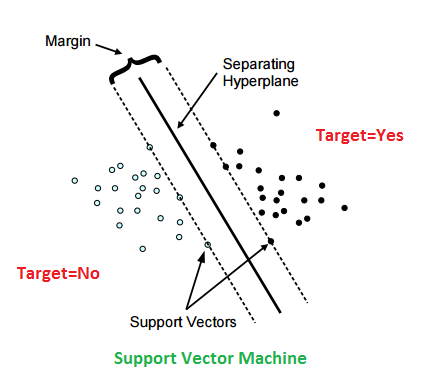
\includegraphics[height=8cm,width=10cm]{SVM-Planes.jpg}
\counterwithin{figure}{section}
\caption{The working principle of SVM.}
%\counterwithout{figure}{chapter}
\end{figure}

\paragraph{}
A good separation between the two possible classes is
achieved by building a maximal margin hyperplane. The
margin maximizes the distance between the classes and
the nearest data point of each class. In general, the larger
the margin is, the lower the generalization error of the
classifier. Figure 2 shows the trade-off margin choice. In
addition, SVMs handles the separation by a kernel
function [18] to map the data into a different space with
a hyperplane. SVM gives the flexibility for the choice of
the kernel, as shown in Figure 3. Linear, polynomial and
radial can be taken as an example for a kernel function.
The choice of a kernel depends on the problem we are
trying to model.
\newpage
\hfill \break
\hfill \break
\hfill \break
\hfill \break
\begin{figure}[H]
\centering
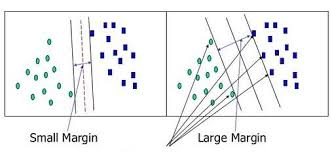
\includegraphics[height=6cm,width=10cm]{image12.jpeg}
\counterwithin{figure}{section}
\caption{the trade-off  margin choice}
%\counterwithout{figure}{chapter}
\end{figure}


\hfill \break
\hfill \break
\begin{figure}[H]
\centering
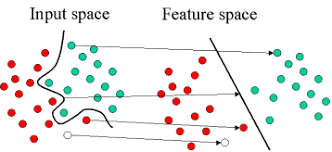
\includegraphics[height=6cm,width=10cm]{download.jpg}
\counterwithin{figure}{section}
\caption{Choice of Kernel function}
%\counterwithout{figure}{chapter}
\end{figure}




\newpage
\section{RESULTS}
\subsection{In static Images}
\paragraph{}
In the sequence of static images in the Cohn-Kanade
datasets, the emotions were detected with a great
accuracy. In this sequence, all images were sorted and
the faces were detected from the haar filters in OpenCV
and were converted to grayscale and were cropped and
were stored. So figure 4 shows some of the images from
the datasets which contained cropped images of faces
only which predicted the emotions perfectly with an
accuracy of 93\% by SVM classification.





\begin{figure}[H]
\centering

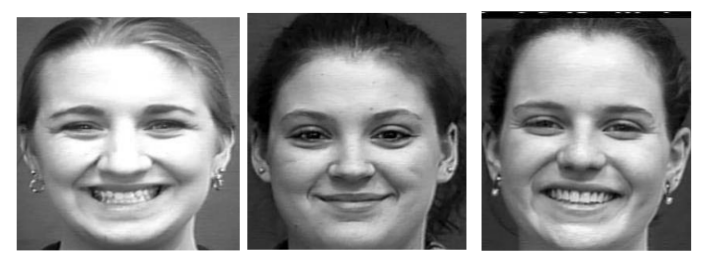
\includegraphics[height=4cm,width=10cm]{happy.jpg}
\counterwithin{figure}{section}
%\counterwithout{figure}{chapter}

\caption{Happy (FACS-0)}
\end{figure}



\begin{figure}[H]
\centering
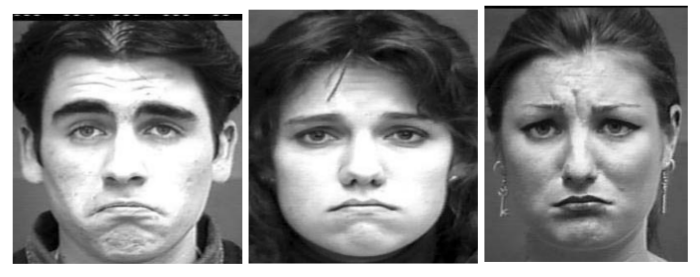
\includegraphics[height=4cm,width=10cm]{sad.jpg}
\counterwithin{figure}{section}
\caption{Sadness (FACS-1)}
%\counterwithout{figure}{chapter}
\end{figure}



\begin{figure}[H]
\centering
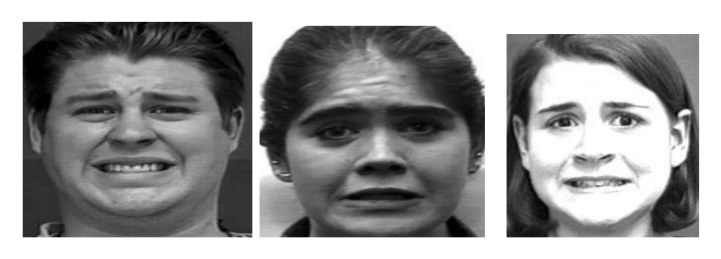
\includegraphics[height=4cm,width=10cm]{fear.jpg}
\counterwithin{figure}{section}
\caption{Fear (FACS-2)}
%\counterwithout{figure}{chapter}
\end{figure}


\begin{figure}[H]
\centering
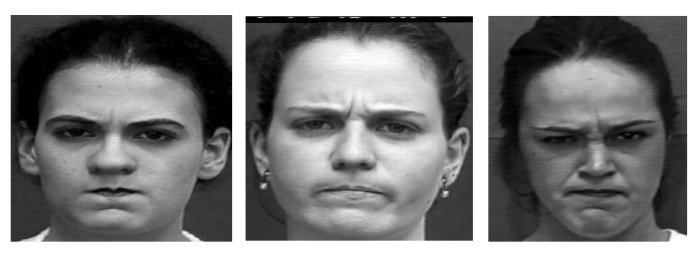
\includegraphics[height=4cm,width=10cm]{angry.jpg}
\counterwithin{figure}{section}
\caption{Angry (FACS-3)}
%\counterwithout{figure}{chapter}
\end{figure}




\begin{figure}[H]
\centering
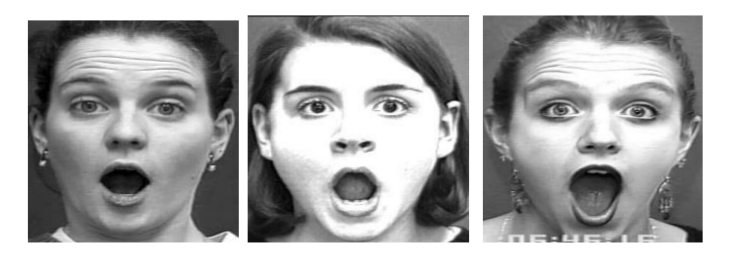
\includegraphics[height=4cm,width=10cm]{surprise.jpg}
\counterwithin{figure}{section}
\caption{Surprise (FACS-4)}
%\counterwithout{figure}{chapter}
\end{figure}

\begin{figure}[H]
\centering
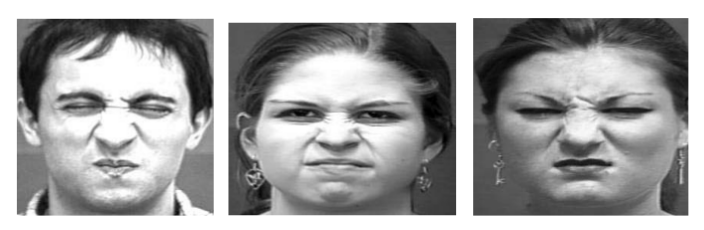
\includegraphics[height=4cm,width=10cm]{disgust.jpg}
\counterwithin{figure}{section}
\caption{Disgust (FACS-5)}
%\counterwithout{figure}{chapter}
\end{figure}

\begin{figure}[H]
\centering
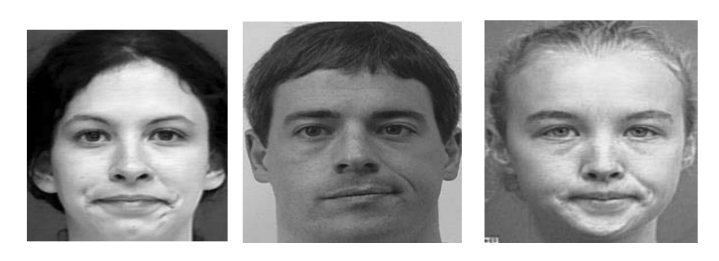
\includegraphics[height=4cm,width=10cm]{contempt.jpg}
\counterwithin{figure}{section}
\caption{Contempt (FACS-6)}
%\counterwithout{figure}{chapter}
\end{figure}

\begin{figure}[H]
\centering
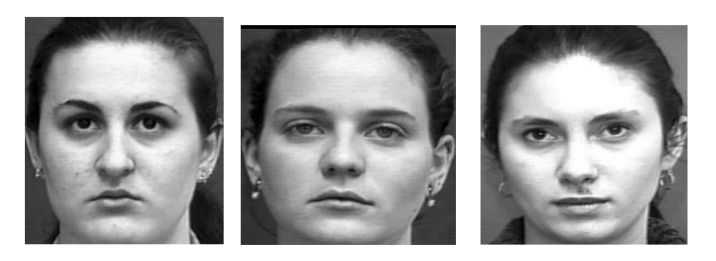
\includegraphics[height=4cm,width=10cm]{neutral.jpg}
\counterwithin{figure}{section}
\caption{Neutral (FACS-7)}
%\counterwithout{figure}{chapter}
\end{figure}

\begin{center}
Fig. 4 The cropped images of faces predicting the
emotions respectively mentioned in (a), (b), (c), (d) (e),
(f), (g), (h), (i).
\end{center}




\paragraph{}
These results show the emotion with their FACS values.
The data was sampled as per 80% training and 20%
testing for high accuracy. In some cases like in the happy
images it was detecting angry or neutral and in surprise
images happy and fear. These were the little errors in the
prediction which reduced the accuracy to 92.1%. But
these small errors are possible when we are dealing with
the large data. The results were stored in different folders
with their emotion names after prediction with their
FACS value within that folder. So this was the automatic
detection of the emotion in static images. We can try
with different datasets and evaluate the accuracy
accordingly.

\subsection{In Real Time}
\paragraph{}
In Real-time the webcam recorded the video and
detected the faces in the yellow box and extracted the
facial landmarks with red dots and then calculated the
centre of gravity with the blue dot [6]. Then the vectors
were calculated with red lines from that centre of gravity
to each and every dot as shown in the figure. The figure
5 shows the screenshot of the results with these facial
landmarks and then predicting the emotion by the SVM
classification [17].

\begin{figure}[H]
\centering
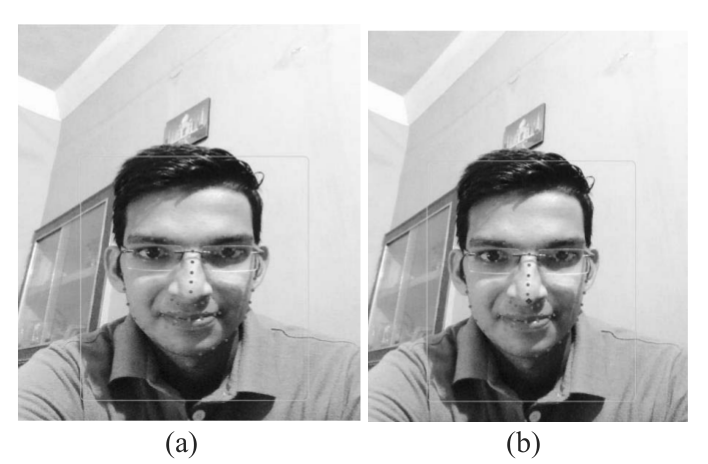
\includegraphics[height=5cm,width=10cm]{realtime1.jpg}
\counterwithin{figure}{section}
\caption{The face detection with the facial
landmarks detected with red dots and centre of gravity.}
%\counterwithout{figure}{chapter}
\end{figure}

\begin{figure}[H]
\centering
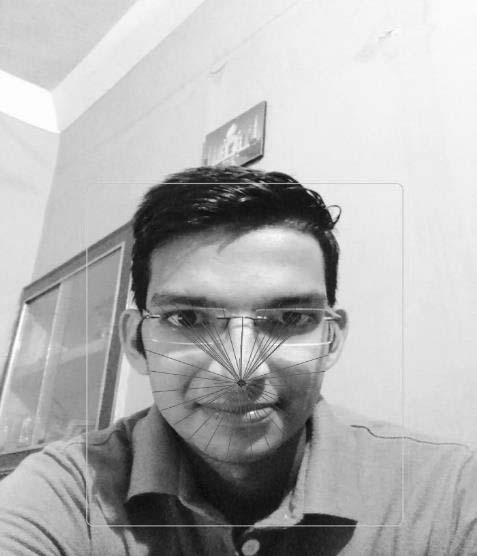
\includegraphics[height=5cm,width=5cm]{realtime2.jpg}
\counterwithin{figure}{section}
\caption{The vectors from COG to every dot}
%\counterwithout{figure}{chapter}
\end{figure}
\begin{center}
(c)
\end{center}


\newpage
\section{DISCUSSION}
\paragraph{}
The linear SVM classification predicted the emotion
with great accuracy. But we also implemented with
polynomial SVM [18] but the accuracy was less than the
linear one. We have also tried with k-means clustering
(unsupervised learning) [14] and Random Forest
Classifier. But in our case SVM were predicting the
emotions with better accuracy as compared to the other
classification algorithms. The tip of the nose can be
chosen as the central point in real time but would
also throw extra variance in the mix due to short, long,
high- or low-tipped noses. Extra variance is
introduced in the “centre point method”; so when the
head moves away from the camera, the centre of gravity
shifts accordingly, but we analyzed this is less than when
we are using the nose-tip method because most faces
more or less face the camera in our sets. The figure 6
shows the screenshot of the output in which the face is
detected in red square and the facial landmarks are
calculated with the red dots with the centre of gravity on
the nose tip with the blue dot. Then the vector lengths
and the angles are calculated as the features extraction.
Then it was trained with SVM. It showed the FACS
value as 4 which means happy. It was tested with
different faces in the real-time with different emotions
on the face it was detecting correctly with an accuracy of
approximately 93.6\%.
\hfill \break
\hfill \break
\begin{figure}[H]
\centering
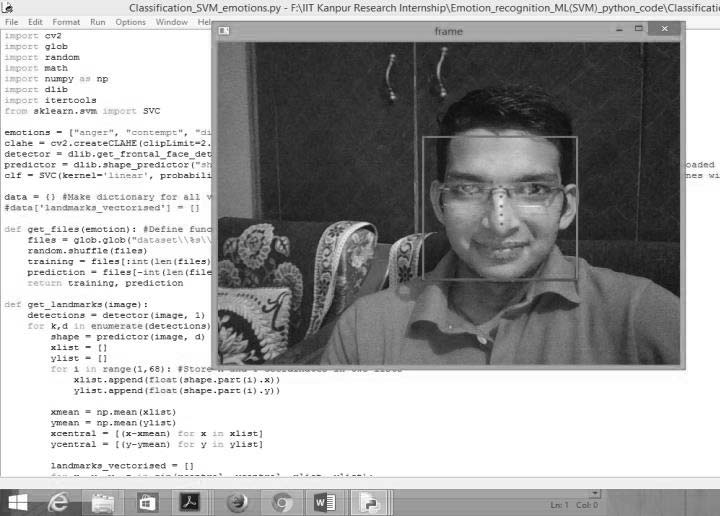
\includegraphics[height=6cm,width=10cm]{Facial-emotion-recognition-in-real-time-and-static-images-031.jpg}
\counterwithin{figure}{section}
\caption{ The face detection with the facial
landmarks detected with red dots}
%\counterwithout{figure}{chapter}
\end{figure}

\newpage
\hfill \break
\hfill \break
\begin{figure}[H]
\centering
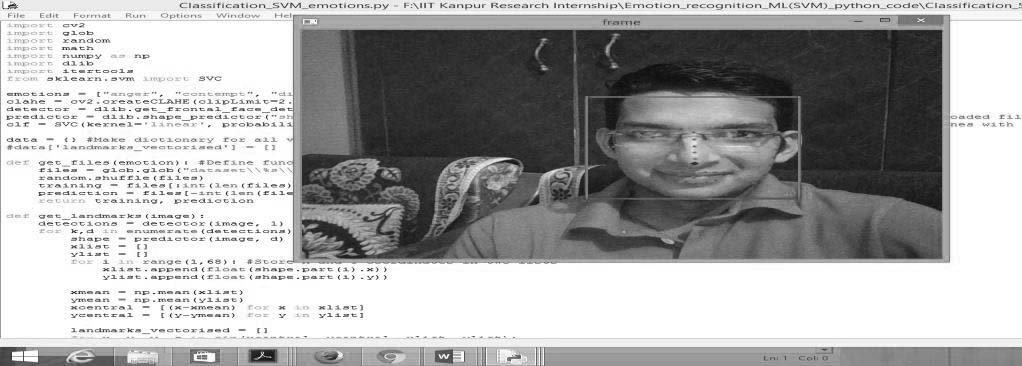
\includegraphics[height=6cm,width=10cm]{Facial-emotion-recognition-in-real-time-and-static-images-032.jpg}
\counterwithin{figure}{section}
\caption{The facial landmarks with the centre of gravity (COG
on Nose Tip)}
%\counterwithout{figure}{chapter}
\end{figure}

\hfill \break
\begin{figure}[H]
\centering
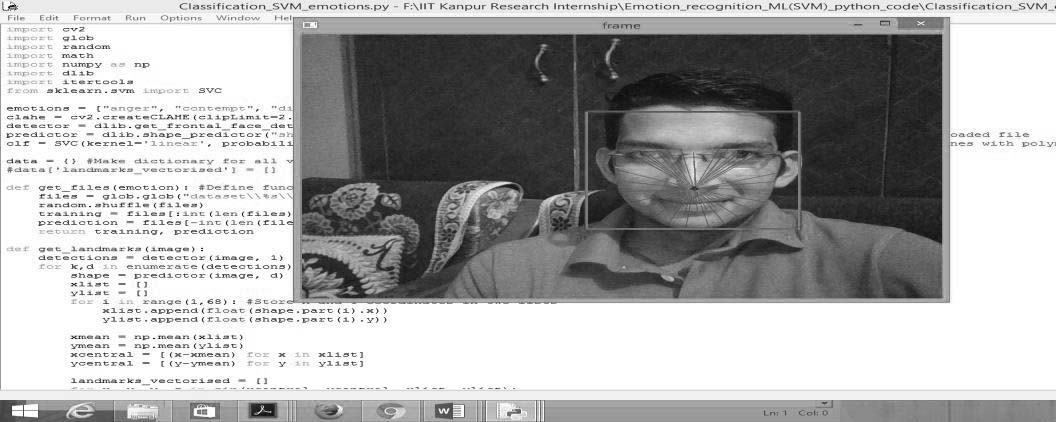
\includegraphics[height=6cm,width=10cm]{Facial-emotion-recognition-in-real-time-and-static-images-033.jpg}
\counterwithin{figure}{section}
\caption{The vectors from COG to every dot}
%\counterwithout{figure}{chapter}
\end{figure}


\newpage
\section{PERFORMANCE EVALUATION}
\paragraph{}
After the detection of the emotions, it is important that
how much accurately our classifier is predicting. So table
1 shows the accuracy in which the column shows the
actual emotion and the row show the emotions predicted
then the accuracy is calculated for every emotion
individually by dividing the number of emotions
correctly detected to the total no of images. So the
overall accuracy was coming around 92.1%. As the
classification is done with different types of
classification algorithms [10]. So table 2 shows the
comparative analysis of accuracy in each case. So we
found that linear SVM was giving the maximum
accuracy of 94.1% when all the features were
considered.

\subsection{In static images}
\paragraph{}

\begin{figure}[H]
\centering
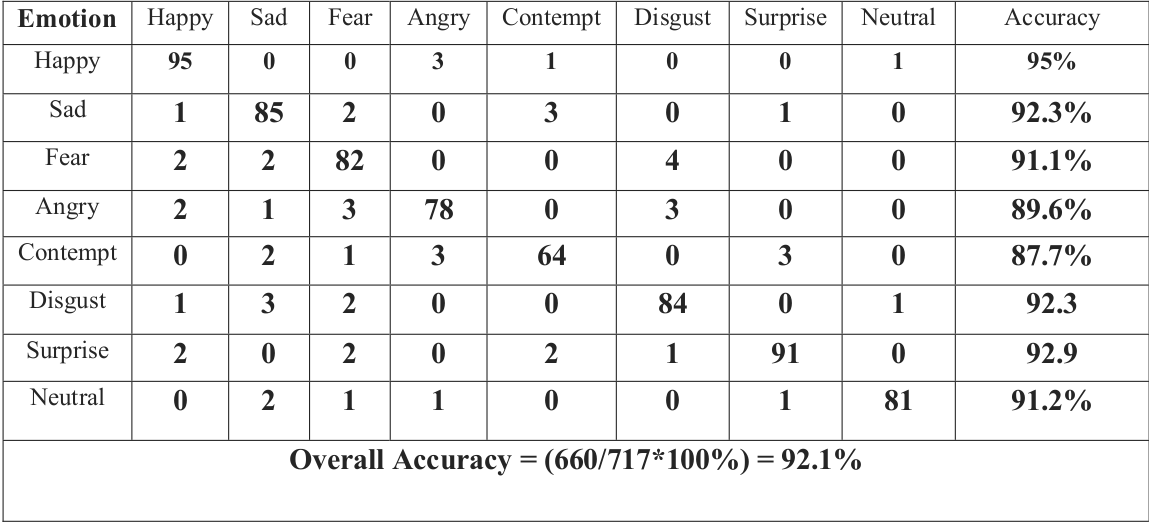
\includegraphics[height=6.5cm,width=12cm]{new1.jpg}
\counterwithin{figure}{section}
\caption{(Table 1 Accuracy for different emotions)}
%\counterwithout{figure}{chapter}
\end{figure}

\subsection{In Real Time}

\begin{figure}[H]
\centering
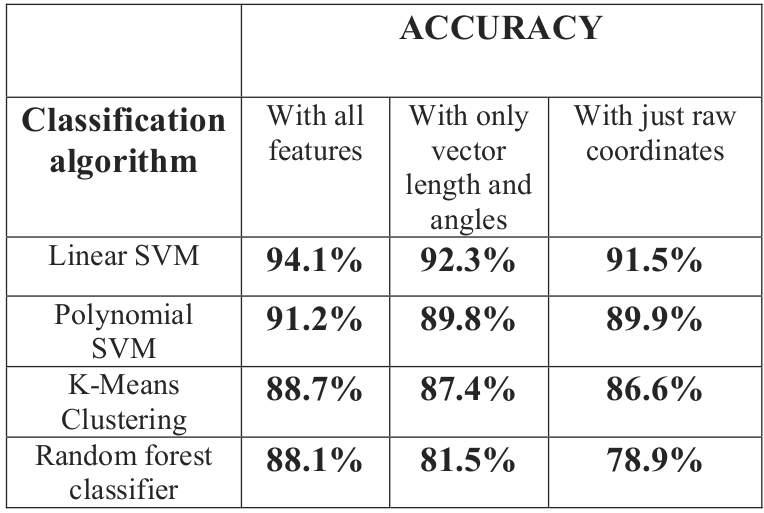
\includegraphics[height=5cm,width=10cm]{new2.jpg}
\counterwithin{figure}{section}
\caption{(Table 2 Accuracy for different classifiers and features.)}
%\counterwithout{figure}{chapter}
\end{figure}


\newpage
\section{CONCLUSIONS AND FUTURE WORK}

\paragraph{}
In this paper, we presented the fully automatic
recognition of facial emotions using the computer vision
and machine learning algorithms which classify these
eight different emotions. We tried many algorithms for
the classification but the best which came out of the
results was the support vectors machines with the
accuracy of around 94.1\%. Our results imply that user
independent, fully automatic real-time coding of facial
expressions in the continuous video stream is an
achievable goal with present power of the computer, at
least for applications in which frontal views can be
assumed using the webcam. This machine learning based
system for the emotion recognition can be extended to
the deep learning system using the Convolutional Neural
networks which will have many layers and the chances
of getting much higher accuracy is there around 99.5\%. This project can be extended in which it will detect
as many emotions of different people in one frame in the
real-time videos [8]. Emotion recognition is going to be
very useful in the near future in the research field of
robotics and artificial Intelligence for example if a robot
can sense the sentiment of any human and that robot can
act accordingly without any intervention of any other
humans. This automatic machine learning system for
emotion recognition can also be extended with the
detection of mixed emotions other than these eight
universal emotions.


\newpage
%\cleardoublepage
\section{REFERENCES}
\begin{thebibliography}{9}


\bibitem{d} Patrick Lucey, Jeffrey F. Cohn, Takeo Kanade, Jason Saragih, Zara Ambadar, \emph{“Recognizing Facial Expression: Machine Learning and Application to Spontaneous Behavior”. }Computer Vision and Pattern Recognition 2005.

\bibitem{d} I. Cohen, N. Sebe, F. Cozman, M. Cirelo, and T. Huang,
\emph{“Learning Bayesian network classifiers for facial expression recognition using both labeled and unlabeled data” }
Computer Vision and Pattern Recognition., 2003.

\bibitem{d}A. Kapoor, Y. Qi, and R.W.Picard.
\emph{"Fully automatic upper facial action recognition."} 
IEEE International Workshop on Analysis and Modeling of Faces and
Gestures., 2003.

\bibitem{d} P. Ekman and W. Friesen,\emph{ Facial Action Coding
System: A Technique for the Measurement of Facial
Movement,”} Consulting Psychologists Press, Palo Alto,
CA, 1978.

\bibitem{d} M. Pantic and J.M. Rothkrantz. \emph{“Automatic analysis
of facial expressions:,”} State of the art. IEEE Transactions
on Pattern Analysis and Machine Intelligence,
22(12):1424–1445,2000.

\bibitem{d} I. Cohen, N. Sebe, A. Garg, L. Chen, and T.S. Huang, \emph{“Facial expression recognition from video sequences:
Temporal and static modeling,”} Computer Vision and
Image Understanding, 91(1-2):160–187, 2003.

\bibitem{d}A.J. Colmenarez and T.S. Huang, \emph{“Face detection with
information based maximum discrimination,” }In IEEE
Conference on Computer Vision and Pattern
Recognition, pages 782–787, 1997.

\bibitem{d} I.A. Essa and A.P. Pentland, \emph{“Coding, analysis,
interpretation, and recognition of facial expressions,”} IEEE Trans. on Pattern Analysis and Machine
Intelligence, 19(7):757–763,1997.

\bibitem{d}M.-H. Yang, D. Kriegman, and N. Ahuja,\emph{ “Detecting
faces in images:,”} A survey. IEEE Trans. on Pattern
Analysis and Machine Intelligence, 24(1):34–58, 2002.

\bibitem{d}Nazia Perveen, Nazir Ahmad, M. Abdul Qadoos
Bilal Khan, Rizwan Khalid, Salman Qadri. ("Facial
Expression Recognition through Machine Learning")International Journal of Scientific \& Technology
Research Volume 5, ISSUE 03, MARCH 2016 ISSN
2277-8616.

\bibitem{d}Ghimire, D., and Lee, J. {"2013, Geometric feature-
based facial expression recognition in image sequences
using multi-class AdaBoost and support vector machines
Sensors,13(6), 7714-7734." }

\bibitem{d} Giorgana, G., and Ploeger, P. G., {"2012, Facial
expression recognition for domestic service robots,
InRobo Cup 2011: "}Robot Soccer World Cup XV, pp.
353-364.

\bibitem{d}Rituparna Halder, Sushmita Sengupta, Arnab Pal,
Sudipta Ghosh, Debashish Kundu {"Real-Time Facial
Emotion Recognition based on Image Processing and
Machine Learning"}International Journal of Computer
Applications (0975 – 8887) Volume 139 – No.11, April
2016.

\bibitem{d}Claudia Lainscsek, Mark Frank, Ian Fasel, Marian
Stewart Bartlett, Gwen Littlewort, Javier Movellan, {"Recognizing Facial Expression: Machine Learning and
Application to Spontaneous Behaviour"}vol. 02, no. , pp.
568-573, 2005, doi:10.1109/CVPR.2005.297


\bibitem{d} Bhuiyan, M. A.-A., Ampornaramveth, V., Muto, S.,
and Ueno, H., {"Face detection and facial feature
localization for human-machine interface. NII Journal,
(5):25–39, 2003."}


\bibitem{d} Philipp Michel, Rana El Kaliouby
{"Real-Time
Facial Expression Recognition in Video using Support
Vector Machines"} ICMI '03 Proceedings of the 5th
international conference on Multimodal interfaces;
ISBN:1-58113-621-8.

\bibitem{d} Amari, S. and Wu, S. (1999) {"Improving support
vector machine classifiers by modifying kernel
functions. Neural Networks, 12(6):783–789."}

\bibitem{d} Bartlett, M., Littlewort, G., Fasel, I., and Movellan,
J., { "(2003). Real-time face detection and facial expression
recognition:" }Development and applications to human-
computer interaction. In Computer Vision and Pattern
Recognition Workshop, 2003. CVPRW

\bibitem{d}  Kotsia, I., Buciu, I., and Pitas, I., {"(2008). An analysis
of facial expression recognition under partial facial
image occlusion"}Image and Vision Computing,
26(7):1052– 106.

\end{thebibliography}

\end{document}